\chapter{Specifikace}

% strana 6 a 9
Sommerville~\cite{sommerville_softwareengineering_2011} uvádí fundamentální aktivity softwarového inženýrství: specifikace, vývoj, validace a evoluce.
Dále definuje softwarovou specifikaci jako aktivitu, při které zákazníci a inženýři definují software, který má být vyprodukován, a omezení na jeho provoz.

V~této kapitole definujeme software, který budeme tvořit, pomocí požadavků uživatele, případů užití, diagramu tříd v~konceptuální vrstvě a procesů.

\section{Požadavky}

Požadavky na softwarový systém jsou popisy toho, co by měl systém dělat -- služby, které poskytuje, a omezení na jeho provoz.
Tyto požadavky by měly reflektovat potřeby zákazníka na systém a jeho účel, uvádí Sommerville~\cite[s.~83]{sommerville_softwareengineering_2011}.

Požadavky na funkce systému nazýváme funkční.
Požadavky na provoz systému a jeho omezení nazýváme nefunkční.

Dále uvedeme vybrané funkční a nefunkční požadavky z~pohledu uživatele systému.

\subsection{Funkční požadavky}
\newlist{enumfp}{enumerate}{1}
\setlist[enumfp]{label=\textbf{FP\hyp{}\arabic*},ref=FP\hyp{}\arabic*}

\subsubsection*{Projekt}
\begin{enumfp}
  \item V systému bude možné vytvořit nový projekt.
  \item Projekt bude možné uložit.
  \item Projekt bude možné načíst.
  \item Projekt bude možné pojmenovat pro odlišení od ostatních projektů.
  \item Jednotlivé diagramy bude možné exportovat do rastrového i vektorového formátu.
  \item Do těchto exportovaných formátů bude volitelně možné vložit projekt, který z nich pak bude možné načíst.
  Tímto bude projekt možné otevřít jak v prohlížeči obrázků (a zobrazit rastrově nebo vektorově diagram), tak v našem systému a pokračovat v práci.
  \item Zobrazení každého diagramu bude možné posouvat myší.
  \item Zobrazení každého diagramu bude možné přibližovat a oddalovat kolečkem myši.
  \item Posunutí a přiblížení bude volitelně možné synchronizovat mezi všemi diagramy.
  \item Systém bude kontrolovat validitu uživatelem vytvořených konstruktů.
\end{enumfp}

\subsubsection*{ER Diagram}
\begin{enumfp}[resume]
  \item Do diagramu bude možné přidat entitní typ.
  \item Do diagramu bude možné přidat vztahový typ.
  \item Do diagramu bude možné přidat atribut.
  \item Mezi entitním a vztahovým typem bude možné vytvořit spojení.
  \item Mezi entitním typem a atributem bude možné vytvořit spojení.
  \item U~spojení bude možné specifikovat a zobrazit kardinalitu.
  Dolní mez bude buď 0 nebo 1, horní mez 1 nebo $n$.
  Výchozí kardinality ($1..1$) nebudou zobrazeny.
  \item Bude možné vytvořit ISA hierarchii mezi entitními typy.
  \item Vlastnosti všech objektů bude možné měnit (popisky, typ, pozice).
  Tyto změny budou reflektovány v~ostatních diagramech.
  \item Objekty bude možné posunovat držením levého tlačítka myši a tažením.
  \item Všechny objekty bude možné zvolit levým tlačítkem myší.
  \item Při držení klávesy \keys{\ctrl} bude možné zvolit více objektů najednou postupným klikáním levého tlačítka myši.
  \item Veškeré objekty bude možné z~diagramu mazat alespoň klávesou \keys{Delete}.
  \item Uživatel bude moct využít předpřipravené konstrukty, které bude možné vložit do diagramu.
  Například se může jednat o~ISA hierarchie s~předpřipravenými entitami.
\end{enumfp}

\subsubsection*{Schématická kategorie}
\begin{enumfp}[resume]
  \item Objekty a morfismy schematické kategorie bude možné přidávat a mazat, přičemž tato změna se odrazí v~ostatních diagramech.
  \item V~diagramu se zobrazí data o~objektech a morfismech včetně kardinalit a popisků.
  Výchozí kardinality ($1..1$) se zobrazovat nebudou.
  \item Objekty bude možné posouvat a jejich posunutí se odrazí na ostatních diagramech.
  \item Při zvolení objektu se barevně vyznačí všechny objekty v~okolí, které ho identifikují (a jinou barvou identifikátory vzdálené).
\end{enumfp}

\subsubsection*{Vizualizace schematické kategorie}
\begin{enumfp}[resume]
  \item Vizualizace schematické kategorie ze schematické kategorie vytěží sémantiku a vizualizuje ji různými tvary.
  \item Při zvolení objektu se barevně zvýrazní bezprostřední a vzdálené identifikátory různými barvami.
\end{enumfp}

\subsection{Nefunkční požadavky}
\newlist{enumnfp}{enumerate}{1}
\setlist[enumnfp]{label=\textbf{NFP\hyp{}\arabic*},ref=NFP\hyp{}\arabic*}

\begin{enumnfp}
\item Aplikaci bude možné používat na všech běžných desktopových operačních systémech.\label{nfp:can-use-everywhere}
  \item Nesmí dojít ke ztrátě práce při náhlém ukončení aplikace kvůli interním či externím vlivům.
  To může být zařízeno např. průběžným ukládáním práce.
  \item Aplikaci bude možné používat i při výpadku internetového připojení.
  \item V~rámci bezpečnosti žádná data týkající se práce na projektu neopustí zařízení klienta, pokud tak klient explicitně neučiní (například export a přesun souboru).\label{nfp:safety}
  \item Aplikace bude navržena tak, aby bylo možné bez větších komplikací rozšířit její funkcionalitu (např. přidat podporu UML).
  \item Aplikace bude nenáročná na provoz a investice provozovatele.\label{nfp:nenarocnost}
\end{enumnfp}

\section{Konceptuální model}

V~této kapitole představíme konceptuální model aplikace.
Jedná se o~část světa, na kterou vymezujeme svůj diskurz.
Využijeme k tomu prostředky \acrfull{uml}~\cite{omg_uml_2017}.

Na Obrázku~\ref{fig:class-diagram:er-diagram} je \acrshort{UML} diagram tříd navrhující konceptuální model \acrshort{er} diagramu.
Obsahuje třídy odpovídající všem konstruktům popsaných v Sekci~\ref{section:entity-relationship} -- entitní typ, vztahový typ, atribut, složený atribut, ISA hierarchie, kardinalita a identifikátor.
Entitní typ, vztahový typ i atribut mají složku vyjadřující jejich uživatelské jméno.
Navíc jsme uvedli tři třídy asociace k asociacím mezi těmito objekty, které mají všechny svou kardinalitu:
\begin{itemize}
  \item \emph{Membership} (členství) vyjadřuje vztah mezi entitním typem nebo vztahovým typem a atributem.
        Toto jméno vyjadřuje, že atributy považujeme za členy (members) entitních a vztahových typů.
        Entitní i vztahové typy mají buď žádný atribut, nebo libovolné množství atributů.
  \item \emph{Composition} (složení) vyjadřuje vztah mezi složeným atributem a atributy, z kterých se skládá.
        Složený atribut musí mít alespoň jeden atribut, jinak ho nepovažujeme za složený.
  \item \emph{Participation} (účast) vyjadřuje vztah mezi vztahovým typem a entitními typy, které se daného vztahového typu účastní.
\end{itemize}

Názvy pro naše tři třídy asociace byly inspirovány \acrshort{er} diagramem, který modeluje \acrshort{er} od Atzeniho~\cite[Obr.~5.22]{atzeni_database_1999}

Tyto tři třídy asociace jsme mohli sjednotit do jedné, protože všechny obsahují pouze jednu instanci kardinality.
Tím by však zanikl jejich rozlišný význam, který může být v určitém kontextu důležitý.
Mohli bychom jim také uvést společného předka, ale to považujeme za zbytečné a konceptuálně nemnoho vypovídající.

Kardinalita se skládá ze dvou složek, jejichž možné hodnoty jsou dány enumeracemi.
To vyjadřuje naše omezení, která jsme na kardinalitu položili.

ISA hierarchie se přesně podle definice skládá z jednoho entitního typu rodiče a jednoho či více entitních typů dětí.
Mohli jsme místo toho modelovat vztah jednoho rodiče s jedním dítětem, ale v \acrshort{er} je důležité nad těmito vztahy uvažovat po $n$-ticích.

Identifikátory jsme namodelovali bez rozlišení významu externích a interních identifikátorů, protože to je vlastnost, která pro každý identifikátor vyplyne až v instanci modelu.
Každý entitní typ musí mít z definice našeho \acrshort{er} modelu alespoň jeden identifikátor (nebo více).
Ten se může skládat z libovolného množství atributů a vztahových typů.
V instanci modelu bychom označili identifikátor mající alespoň jeden vztahový typ jako externí, jinak interní.
Přestože model technicky povoluje i identifikátory bez členů, nejsou takové identifikátory validní.

Na Obrázku~\ref{fig:class-diagram:schemcat} je konceptuální model schematické kategorie.
Stěžejními třídami v modelu jsou objekt, morfismus a signatura.

Signatura se skládá z jednotlivých symbolů, kterých může být 0 (prázdný řetězec $\varepsilon$) a více.
Jedná se totiž z Definice~\ref{def:signature} o řetězec.
Jednotlivými symboly může být úplně cokoli, dle volby abecedy.
Podle volby v implementaci může jít o znaky, řetězce, či libovolné objekty.
Signatury lze řetězit za sebe, což jsme vyjádřili operací \texttt{concat}\footnote{z anglického \emph{to concatenate} -- zřetězit, spojit},
která vrátí novou signaturu vzniklou zřetězením této a jiné, předané parametrem \texttt{other}.
Pokud označíme danou instanci signatury \texttt{tato}, zřetězení by mělo probíhat v pořadí \texttt{tato} $\cdot$ \texttt{other}, stejně jako je to běžné u jazyků.
Až v implementaci by se mělo dbát na správné pořadí při skládání morfismů, které je opačné.

V konceptuálním modelu vyjadřujeme, že každý objekt musí mít alespoň jeden identifikátor, který se skládá ze signatur.
Speciálně tímto identifikátorem může být i $\set{\set{\varepsilon}}$, protože signatura může být prázdný řetězec.
Jak jednotlivé identifikátory, tak celá jejich sada u daného objektu, by měla být množina, a proto se nemusí dbát na pořadí a duplicity.

Pro morfismy je vyjádřeno, že by měl mít každý svou signaturu.
Mohli bychom morfismy vydělit na námi definované druhy specializováním třídy morfismu na bázový, odvozený a identitní.
U bázových by bylo vyjádřeno, že jejich signaturou je pouze jediný symbol.
U odvozených je jejich signaturou již namodelovaná třída signatury.
A u identitních je jejich signaturou prázdný řetězec, tedy konstanta.
Toto rozdělení nám však pro konceptuální model přijde zbytečné, protože se jedná o vlastnost morfismu, která vyplyne z toho, z kolika symbolů se jeho signatura skládá.

Další prvky konceptuálního modelu schematické kategorie jsou zřejmé a vycházejí přímo z definice schematické kategorie ze Sekce~\ref{section:schemcat}.

Konceptuální model \acrfull{vsk}, který je na Obrázku~\ref{fig:class-diagram:scv}, je podobný konceptuálnímu modelu schematické kategorie, s několika málo rozdíly.
Koncept signatury ve vizualizaci zaniká.
Místo toho jsou identifikátory objektů tvořeny přímo navazujícími morfismy.
Objekty a morfismy ztrácí svoji identitu, resp. signaturu.
Ta konceptuálně ve \acrshort{vsk} není.

V konceptuálním modelu \acrshort{vsk} nově rozlišujeme dva typy objektů -- self-identifikovaný objekt (definovaný v Sekci~\ref{section:vsk}) a naproti tomu externě identifikovaný objekt.
Rozlišujeme je kvůli tomu, že ve \acrshort{vsk} jsou zobrazeny různými tvary.

Protože ve \acrshort{vsk} zanikají inverzní morfismy, mizí z konceptuálního modelu v morfismu i složka udávající směr.

Doména a kodoména nejsou ve \acrshort{vsk} konceptem a mohli bychom je pojmenovat např. zdrojový a cílový objekt.
Nicméně pro přehlednost a snahu o menší komplikaci konceptuálních rozdílů ponecháme i ve \acrshort{vsk} názvy doména a kodoména.

Další koncepty jsou totožné konceptuálním modelem schematické kategorie.

\begin{figure}[!htb]
  \centering
  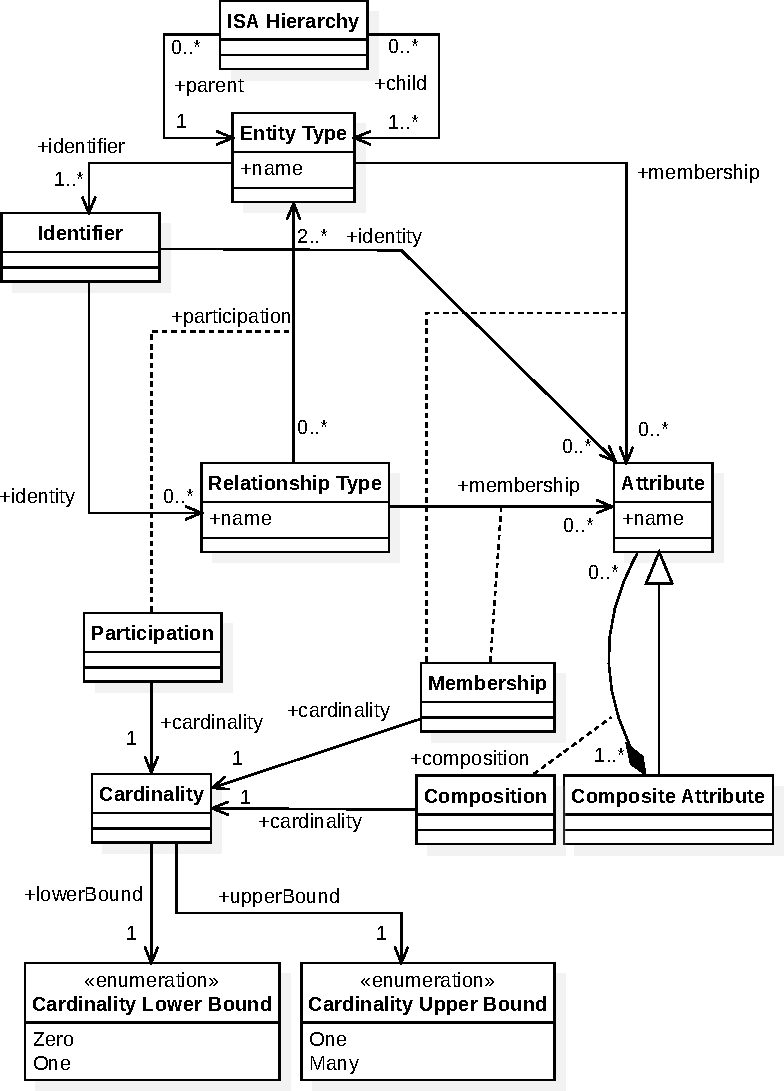
\includegraphics[width=\maxwidth{\textwidth}]{../img/diagrams/er-diagram-model.pdf}
  \caption{Diagram tříd -- ER diagram}
  \label{fig:class-diagram:er-diagram}
\end{figure}
\begin{figure}[!htb]
  \centering
  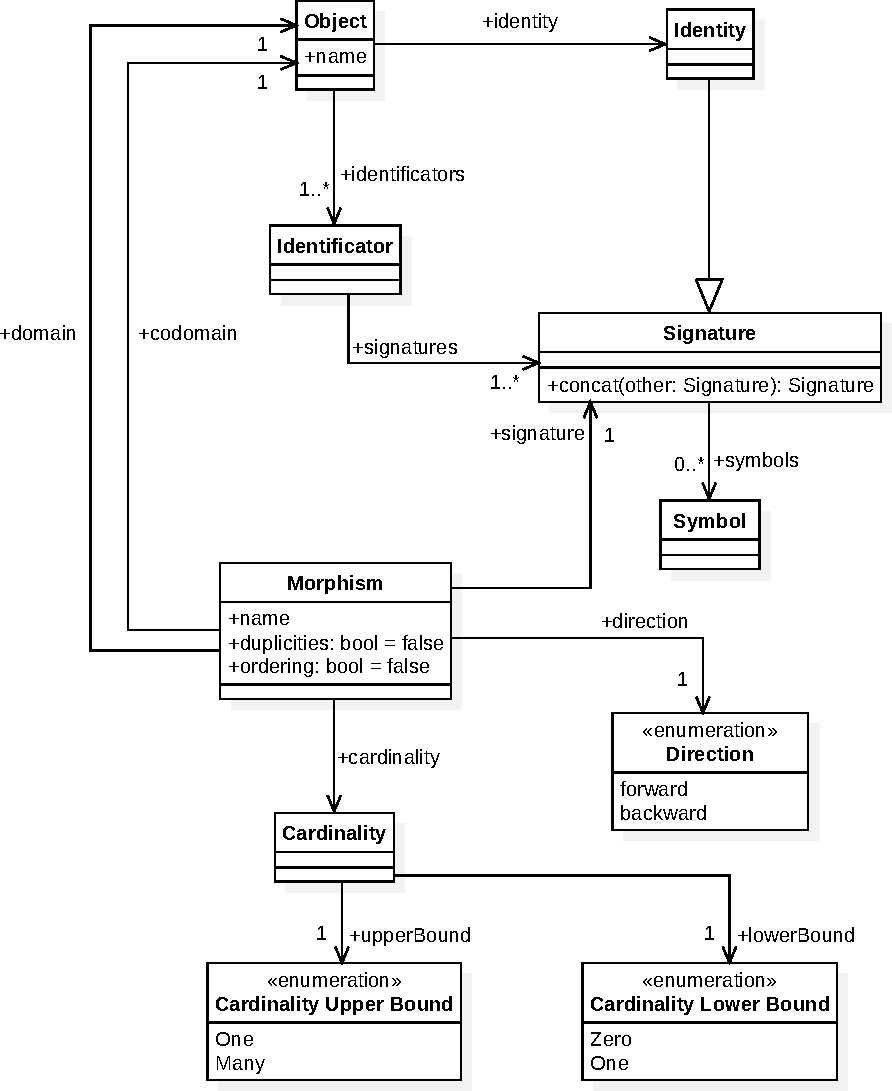
\includegraphics[width=\maxwidth{\textwidth}]{../img/diagrams/schema-category-model.pdf}
  \caption{Diagram tříd -- schematická kategorie}
  \label{fig:class-diagram:schemcat}
\end{figure}
\begin{figure}[!htb]
  \centering
  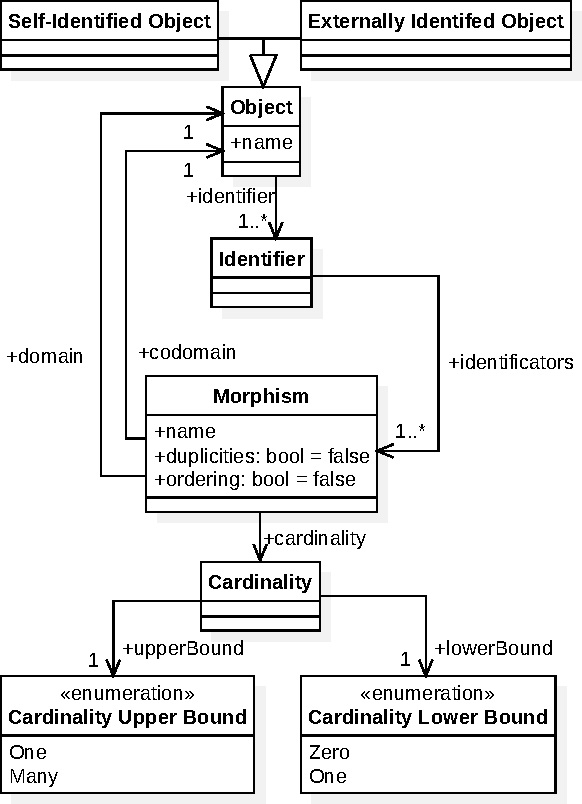
\includegraphics[width=\maxwidth{\textwidth}]{../img/diagrams/scv-model.pdf}
  \caption{Diagram tříd -- \acrlong{vsk}}
  \label{fig:class-diagram:scv}
\end{figure}

\section{Případy užití}

Případy užití definují funkcionalitu systému a reprezentují se diagramem případů užití (use case diagram).
Každý případ užití popisuje jeden způsob, jak lze systém použít.
Uživatelé systému (lidé, stroje, nebo jiné systémy) jsou v diagramu reprezentováni tzv. herci (actors).
Model tak popisuje způsoby, kterými lze systém použít jeho okolím a jaké služby systém nabízí.~\cite[s.~65]{overgaard_usecases_2005}

Případy užití rozdělíme do několik okruhů.
Jedním okruhem je funkcionalita diagramů a jejich plátna, která je u všech diagramů téměř stejná.
Dále vydělíme funkcionalitu části systému, který se stará o správu projektu jako celku.

\begin{figure}[!htb]
  \centering
  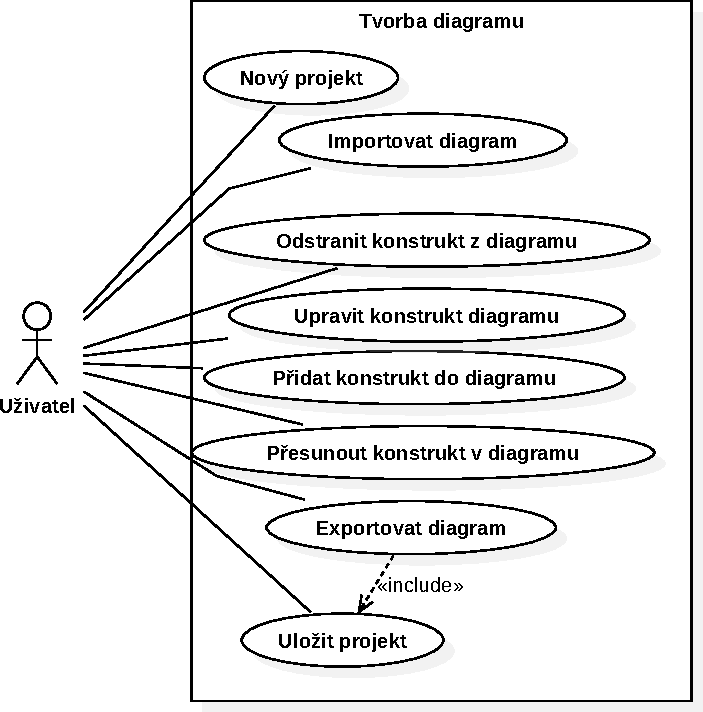
\includegraphics[width=\maxwidth{0.7\textwidth}]{../img/diagrams/use-case-diagram.pdf}
  \caption{Diagram případů užití}
  \label{fig:use-case-diagram}
\end{figure}

\section{Koncept řešení}

Zejména kvůli požadavku~\ref{nfp:can-use-everywhere} za řešení volíme webovou aplikaci.
Kvůli požadavkům~\ref{nfp:nenarocnost} a~\ref{nfp:safety} se však bude jednat o statickou webovou aplikaci.

Statická webová aplikace se stahuje ze serveru jen při přístupu uživatele do aplikace.
Dále už prohlížeč uživatele se serverem nijak nekomunikuje.
Díky tomu bude aplikace nenáročná na provoz, protože stačí statický webový server, který ji pouze zpřístupní v prohlížeči.

Dále je vhodné, že každé moderní desktopové zařízení s téměř libovolným desktopovým operačním systémem disponuje webovým prohlížečem.
Tím umožníme nezávislost na cílové platformě zařízení, protože naší platformou bude právě webový prohlížeč.

Aby se jednalo o statickou webovou aplikaci, server musí umět pouze odesílat webové stránky uživateli.
Výsledný formát aplikace musí být tedy soubory webových technologií, které se budou bez úprav odesílat do prohlížeče uživatele.
Docílí se toho překladem z moderních webových technologií vyššího řádu do starších webových technologií nižšího řádu (HTML, JavaScript, CSS).

Programovací jazyk zvolíme TypeScript vytvořený společností Microsoft~\cite{microsoft_typescriptjavascript_2023}.
Tento jazyk je nadstavbou JavaScriptu, která přidává mj. statické typové kontroly.
Statické typové kontroly umožňují udržitelnost větších projektů, protože vytváří kontrakty mezi částmi aplikace (např. typy parametrů funkce), na rozdíl od JavaScriptu, který je dynamicky typovaný.
Kontroly se uskutečňují při překladu do JavaScriptu.

Jako framework zvolíme React od společnosti Meta Open Source~\cite{react_2023}.
Jedná se o framework pro tvorbu webových aplikací a uživatelských rozhraní, který používá vývojové paradigma tzv. komponent.
Idea je taková, že vývojář vytváří malé komponenty, které skládá do větších komponent, z kterých nakonec složí webovou aplikaci.
Pod komponentou si lze představit nějaký ovládací prvek uživatelského rozhraní, např. tlačítko, nebo např. entitní typ z \acrshort{er}.
React podporuje TypeScript, což odpovídá našemu zvolenému programovacímu jazyku.
Tento framework byl v roce 2022 nejpoužívanější front-end webový framework~\cite{stackoverflow_developersurvey_2022}.
Tím máme zaručenu velkou komunitu vývojářů a velký výběr knihoven.

Diagramy budeme vykreslovat pomocí SVG~\cite{brinza_svg_2018}.
To je přímo podporované v HTML většinou moderních webových prohlížečů.

Hlavní komponentou aplikace bude SVG plátno, ve kterém budou položené komponenty jednotlivých konstruktů diagramů, které budou složeny ze SVG tvarů.
Kromě pláten budeme potřebovat modul s uživatelskými prvky, jako jsou tlačítka pro menu a ovládací prvky pro změnu vlastností konstruktů v diagramech.
Posledním hlavním modulem, bude modul s modelem aplikace, obsahující nejrůznější třídy a rozhraní, které budou odpovídat jednotlivým konstruktům a diagramům.
